%----------------------------------------------------------------------------------------
%	PACKAGES AND DOCUMENT CONFIGURATIONS
%----------------------------------------------------------------------------------------
\documentclass[a4paper,11pt]{article}
\usepackage{amsmath} % Required for some math elements
\usepackage{hyperref} 
\usepackage{xcolor}
\usepackage{lipsum} 
\usepackage{cite}
\usepackage{graphicx} % Required for the inclusion of images
\usepackage{algorithmic}
\usepackage{array}
\usepackage{bookmark}
\usepackage{listings}
\usepackage{mcode}
\usepackage{amssymb}
\usepackage{enumitem}
\usepackage[margin=16mm,]{geometry}
\usepackage[caption=false, font=footnotesize]{subfig}

\newlist{steps}{enumerate}{1}
\setlist[steps, 1]{label = Step \arabic*:}

\hypersetup{ %color attributes of citation, link, etc.
    colorlinks=true,
    linkcolor=blue,
    filecolor=gray,      
    urlcolor=blue,
    citecolor=blue,
}

\newcommand{\matlab}{\textsc{Matlab }} %very important and totally necessary addition

\newcommand\Item[1][]{%
  \ifx\relax#1\relax  \item \else \item[#1] \fi
  \abovedisplayskip=0pt\abovedisplayshortskip=0pt~\vspace*{-\baselineskip}}
  %----------------------------------------------------------------------------------------
%	DOCUMENT INFORMATION
%----------------------------------------------------------------------------------------
 
\title{ECEN315 LABORATORY REPORT TWO}
\author{Daniel Eisen : 300447549}
\date{\today}

\begin{document}
\maketitle
\section*{\small{\textit{Abstract}}}
\small{\textit{The aim of this project was to model the complex system on a DC motor driven compound pendulum and to design an adequate controller to set the pendulum at set angle effectively - measurements in terms of overshoot, settling time and oscillations (around setpoint).
The inter-block relationships of the system were measured and linearly approximated were necessary.
The open loop simulation was constructed and compared to the theoretical model.
The system was then closed, evaluated and the controller designed. This control was successful in eliminating overshoot, removing oscillations and improving the systems settling time (sub 2s).}}

\section{Introduction}
As a follow on from the previously constructed theoretical model of the driven pendulum system, the system is reconstructed in Simulink and the Simscape power systems ecosystem as a (more accurate) representation of the system. This requires calibration of internal relationships that will allow for the design of a PID based compensator to be implemented in order to better control the behaviour of the pendulum when in operation, ideally illuminating the overshoot, oscillations, steady state error and slow settling time all present in the open loop response of the system.

\section{Background}
\textit{\textbf{PID Controller - }} the proportional–integral–derivative is a mechanism for applying correction within a system in feedback. Where the input to the PID controller is the error ($e$), difference between desired setpoint and measured output and the output correction is the sum of 3 proportional, integral, and derivative terms (denoted $P (K_p)$, $I (K_i)$, and $D (K_d)$).\\

\textbf{P} term has an output just linearly proportional to he input error:
$$K_p \cdot e(t)$$
This is where the system is driven in proportion to the current error, i.e. a large gain will result in a large response to small error and vis versa. This method however propagates steady state error.

\textbf{I} term responds to both the size and duration of the error, multiplying this accumulated offset by the error.
$$K_i \int_{0}^{T} e(t) $$
This accelerates the movement of the process towards setpoint and eliminates the steady-state error that occurs with a P controller. Though it cause overshoot with these as it accurate this error.

\textbf{D} term is reactive to the rate of change of the system error, with its response determined by $K_d$
$$Kd\cdot \frac{d}{dt}e(t)$$
This works by trying to anticipate the motion of the system. But is susceptible it applying high frequency gain and noise.


\newpage
\section{Methodology and Results}
\subsection{Open-Loop Control}
In order to facilitate the reconstruction of the system for use in Simulink [with the provided library block] the relevant relationships between input types and outputs must be calibrated. This will be used to setup the control scheme to allow for an angle to be input as a target and for the later auto-automatic control when closing the loop.
\subsubsection{Voltage/Angle Relationship}
Initially, to enable an angle input, the relationship between input voltage to output steady-state angle [of the driven pendulum] needs to be obtained. \\

{\centering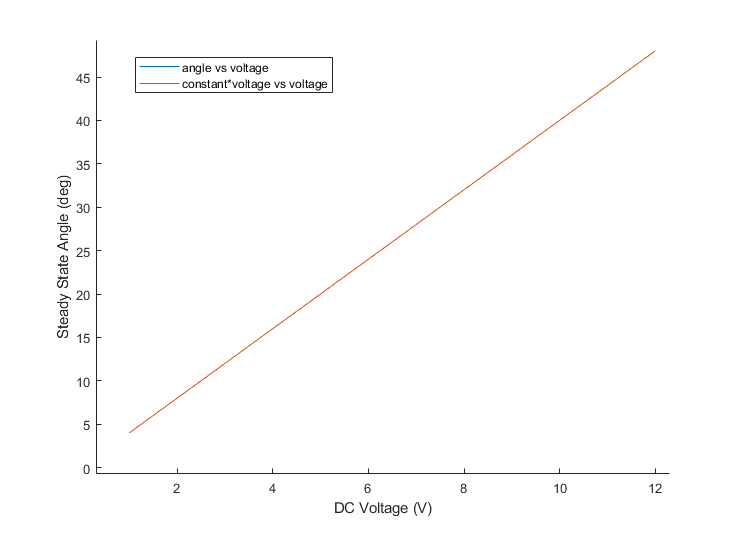
\includegraphics[width=0.5\textwidth]{inc/angle_v_volt.png} \\}
\begin{center}
        Figure 1. Direct DC Voltage VS Steady-state Angle
\end{center}

Varying of the output voltage of the power supply, directly driving the pendulum and taking measurements of the achieved steady state angle(\matlab automation code and Simulink model(s) are in appendix 1). Figure 1 shows the results of this procedure, indicating a linear relationship between the input voltage and output angle (steady-state). From this data a constant was derived, Angle to Voltage $=0.2498$, and its reciprocal for vis versa. 

\subsubsection{PWM Driving}
In practice the pendulum will not be driven by a direct DC voltage, but via a PWM motor driver connected with a Arduino (or similar microcontroller). This "pulse width modulation" method of motor control is far more efficient than the direct method and the modulation refers to the controller changing the duty cycle ($D$) of a generated square wave with amplitude $V_{max}$ to deliver a specified equivalent DC voltage. $V_{eqvDC} = D{\cdot}V_{max}$\\

In this system this duty cycle is determined be an input, $V_{ref}$, which represents an 8bit resolution reference value to set a duty cycle of the driver.\\

In order to control the system it is required to establish/calibrate the relationships between required voltage (to get an angle), the needed duty-cycle to achieve the equivalent voltage, the the PWM reference value to get that duty cycle.

\begin{table}[h]
        \centering
        \begin{tabular}{|l|l|l|l|l|l|l|l|l|l|l|}
        \hline
        0.0 & 0.094 & 0.187 & 0.315 & 0.421 & 0.501 & 0.589 & 0.675 & 0.746 & 0.840 & 0.933 \\ \hline
        \end{tabular}
        \caption{Measured Duty Cycle values from set PWM references}
\end{table}

To establish these relationships the driver was given a range of $V_{ref}$ from 0-250 and the duty cycle read from the scope measurements, Table 1 holds these. A \matlab script then computes the relationship between $D$ and $V_{ref}$, $262.13$ and plots the resultant effective voltage against the $V_{ref}$.

{\centering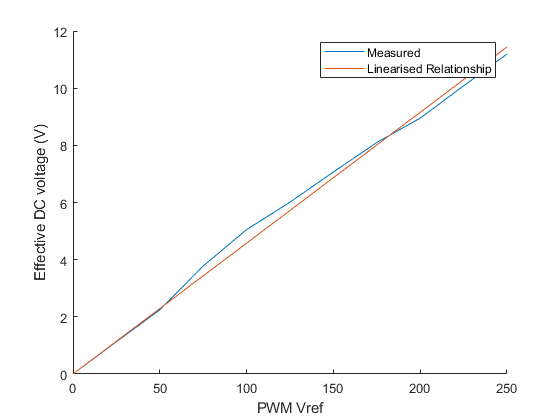
\includegraphics[width=0.45\textwidth]{inc/PWN_effDC.png}
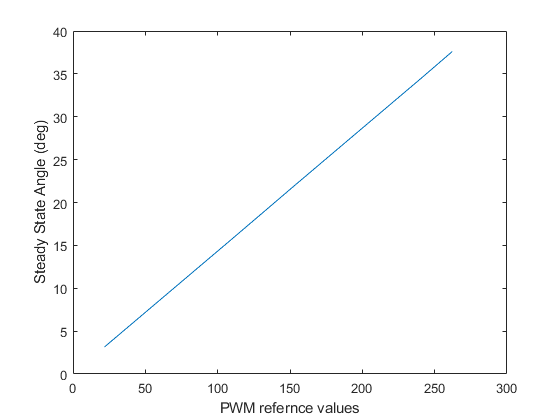
\includegraphics[width=0.45\textwidth]{inc/angle_v_pwm.png}\\}
\begin{center}
        Figure 2. Measured Duty Cycle \hspace{16mm} Figure 3. Results of PWM driven system.
\end{center}

Figure 2. shows the results of the duty cycle measurements and the resultant linearised relationship, and Figure 3. shows the simulation [from section 3.1.1] rerun but with PWM driven for the same equivalent voltages. 

\subsubsection{Incorporation and testing}
Setting up system for wanted angle in and steady state angle out, and testing the result of the established relationships above, with and without internal system error. Firstly in order to use the potentiometer output as feedback into the upcoming closed loop or at least have it properly represent the pendulum angle, a gain between the two must be measured. This was done by comparing the steady state value of both the applying the necessary controller to match, found value of 0.04 (See appendix).

With every relationship determined the open loop system can be constructed to allow for and input angle and a output angle read from the potentiometer, (see system in appendix), with 3 input gain controllers [angle $\Rightarrow$ voltage$\Rightarrow$ duty cycle $\Rightarrow$ PWN $V_{ref}$] and the prior discussed pot output scaler. This can then by tested and the exact angle to voltage relationship tuned in to the right value, and compare its response with and with out error (introduced in the driver).

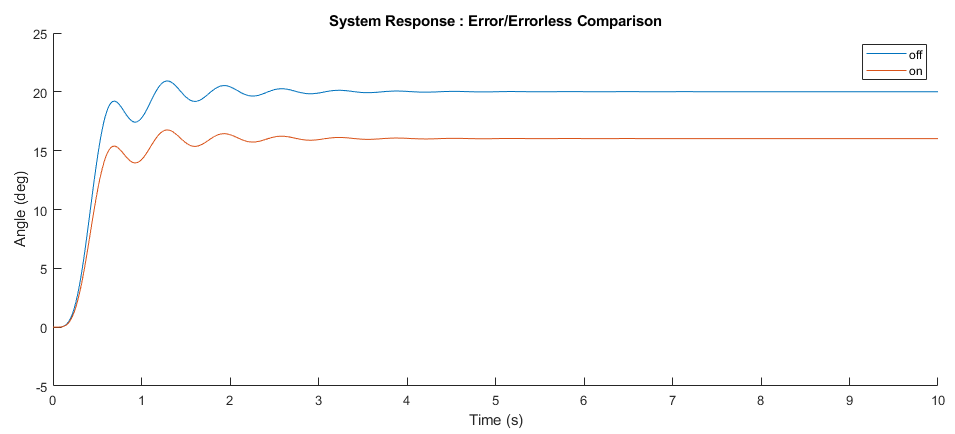
\includegraphics[width=0.9\textwidth]{inc/openloop_response.png} 
\begin{center}
        Figure 4. Error/Errorless response for 20$^\cdot$ set point
\end{center}

As shown in Figure 4. the open-loop meets the required steady state without error, but does not with introduced error, see appendix for measured results.

\newpage
\subsection{Closing the Loop}
\subsubsection{Theoretical Model}
\begin{align*}
        \frac{\Theta(s)}{V(s)} &= \frac{\frac{K_t}{L_aJ_m}}{s^2 + \frac{R_{a}J_{m} + L_{a}D_{m}}{L_{a}J_{m}}s + \frac{R_aD_m + K_tK_b}{L_aJ_m}} \cdot K_{p} \cdot r \cdot \frac{\frac{1}{J_{p}}}{s^{2} + \frac{c}{J_{p}}s + \frac{mgd}{J_{p}}} \\
        &= \frac{rK_pK_r}{as^4+bs^3+cs^2+ds+e}
\end{align*}

\begin{align*}
s.t: \\
a &= L_aJ_mJ_p\\
b &= J_p(R_{a}J_{m} + L_{a}D_{m})+cL_aJ_m\\
c &= mgdL_aJ_m + J_p(R_aD_m + K_tK_b)+c(R_{a}J_{m} + L_{a}D_{m})\\
d &= c((R_aD_m + K_tK_b) + mgd(R_{a}J_{m} + L_{a}D_{m})\\
e &= c(R_aD_m + K_tK_b)
\end{align*}
When loop closed $e_{closed} = e + rKpKt$ \\

\textbf{Evaluation:}\\
        
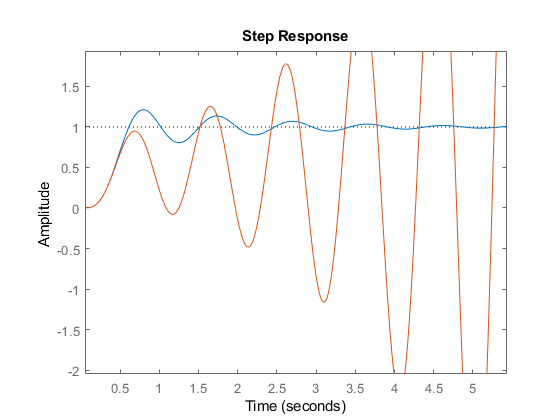
\includegraphics[width=0.3\textwidth]{inc/theory_step.png}
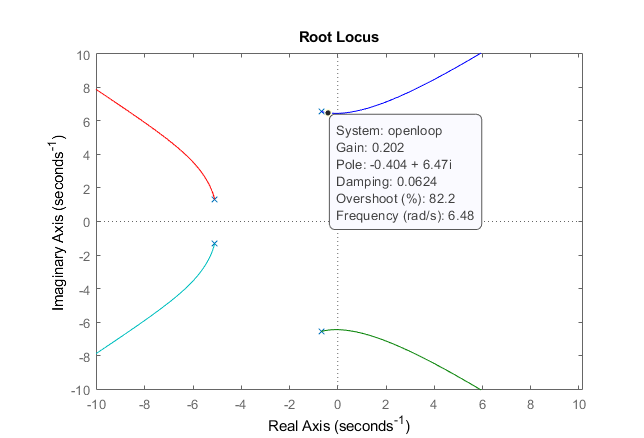
\includegraphics[width=0.3\textwidth]{inc/theory_rlocus.png}
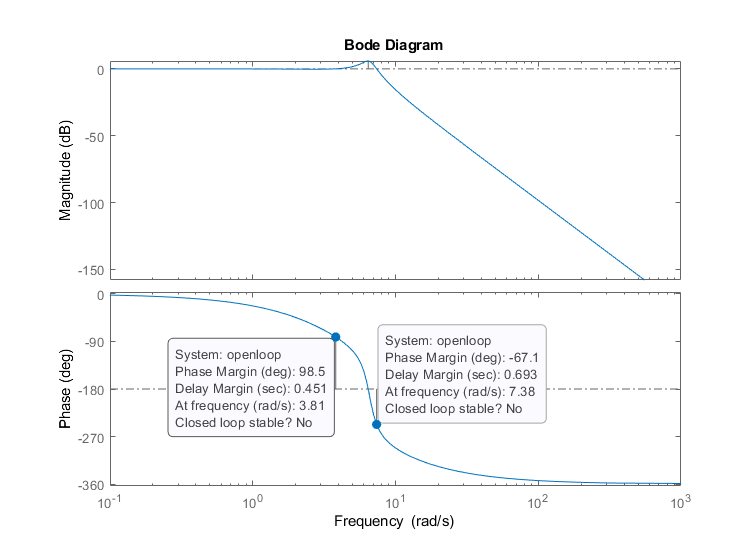
\includegraphics[width=0.3\textwidth]{inc/theory_bode.png}

Various methods can be used to evaluate the potential closed loop response of the system (in theory). A Step response shows the closed system is not stable at a gain of 1. A root locus analysis indicates a narrows band of stable gain values less than 0.04 but most importantly a bode plot shows the phase margin at 7rad/s os -67.1. very far from closed loop stable.


\subsubsection{"Practical" Construction}
Constructing the "actual" system in Simulink with electrical Simscape components (appendix) examining at various Kp gains shows the actual system is more stable at higher gains, but still highly oscillatory, unstable at Kp larger than 1.5 and slow. \\

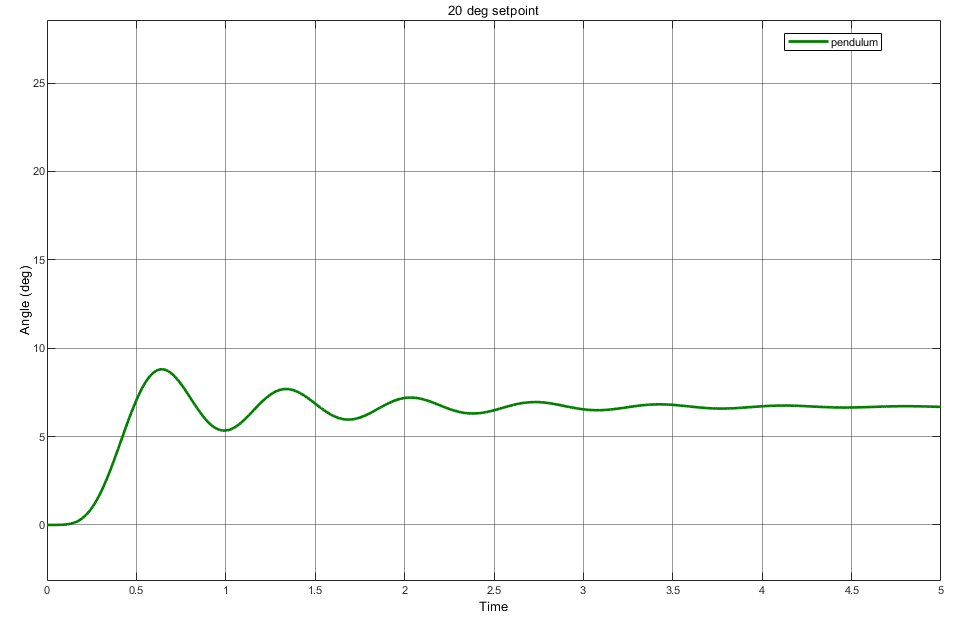
\includegraphics[width=0.3\textwidth]{inc/closedKP05.png}
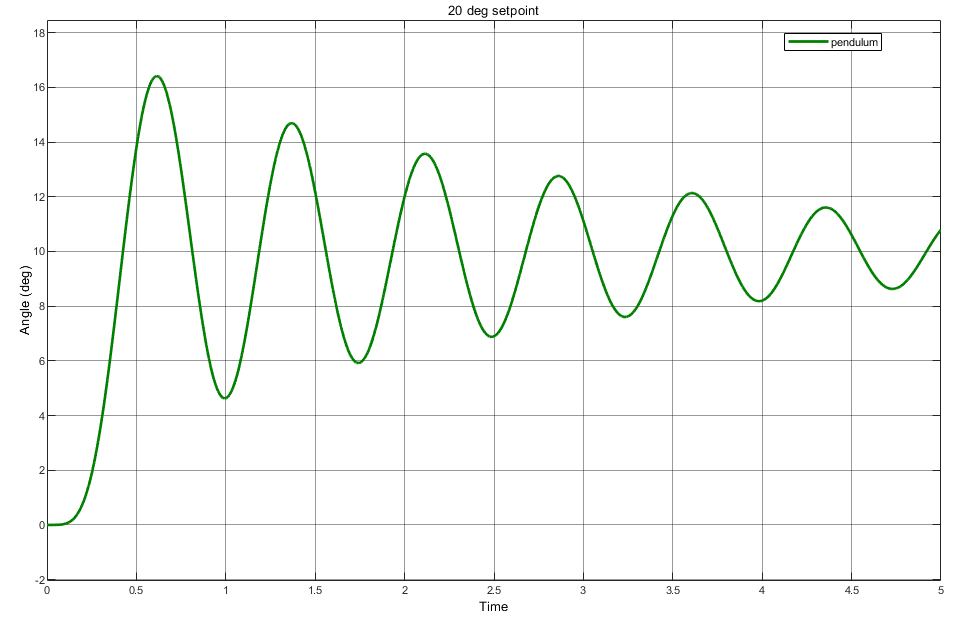
\includegraphics[width=0.3\textwidth]{inc/closedKP1.png}
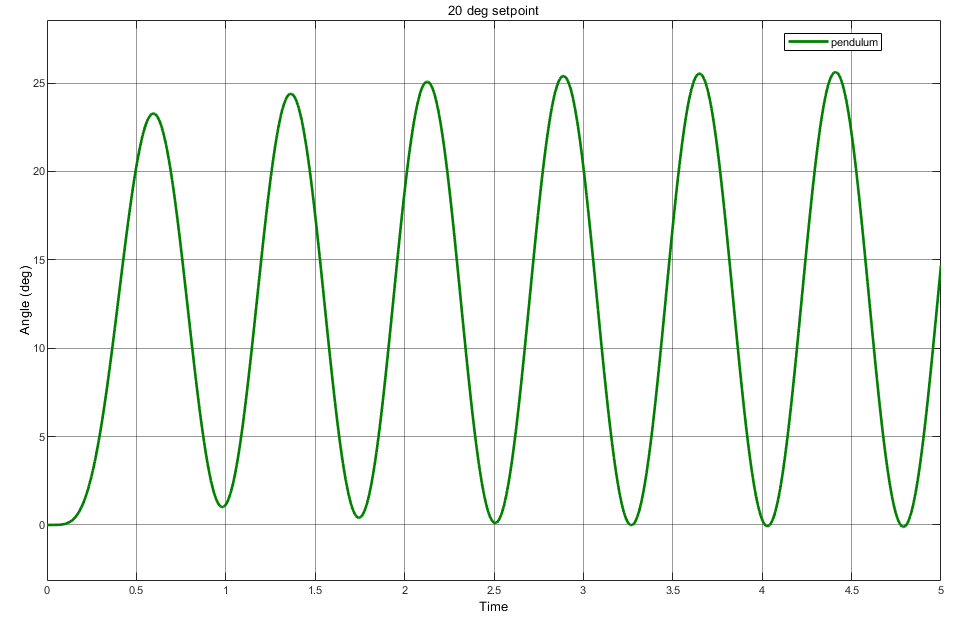
\includegraphics[width=0.3\textwidth]{inc/closedKP15.png}

\newpage
\subsection{PID Control}
To now stabilise and control the closed loop system, as well as eliminate steady state gain, Proportional–Integral–Derivative (PID) compensation is introduced as described in the background.
The system (now closed) begins stable for $K_p$ under 1.5 but highly oscillatory with high SSE. Initially each term of the compensator is designed to achieve each of their provided affect, then combine and tune for final system.

(See appendix for model)

\subsubsection{Pre-design}

{\centering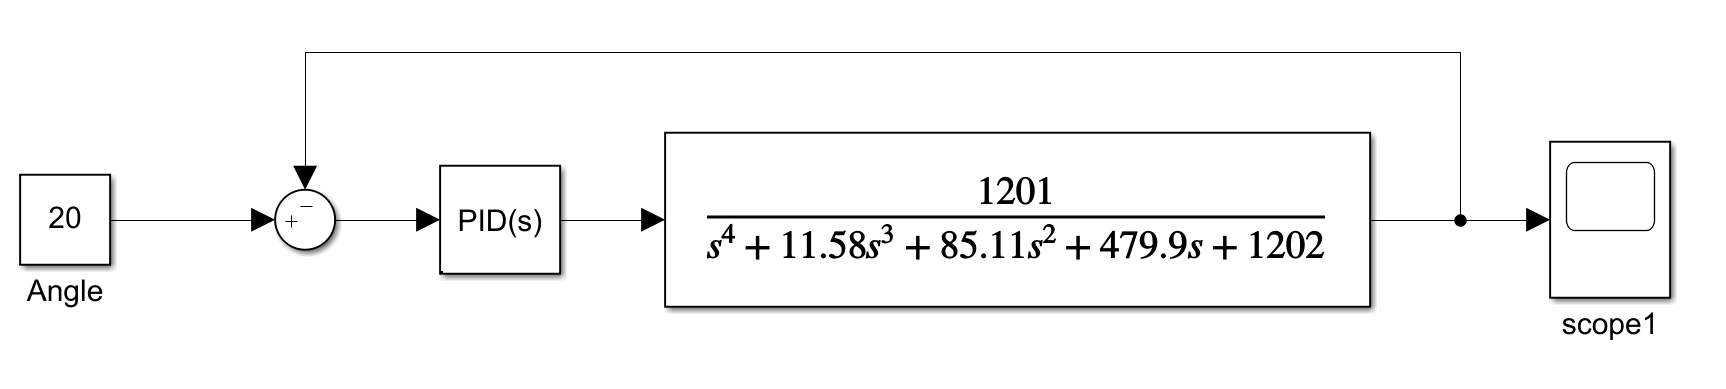
\includegraphics[width=0.75\textwidth]{inc/lab3_pid.png}\\}
\begin{center}
        Figure 5. Lab 3 Theoretical TF in closed PID loop
\end{center}
The first step taken to get an understanding of the real system, was to import the theoretical model into Simulink and using the PID tuning block to understand how initial values for the PID system affect the speed of response, robustness and stability of the system. This providing rough values of $P=(0,0.2), I=(1.5,1.7), D=(0,-0.06)$ (see appendix for response), this gave a fast but still quite oscillatory response but given that the theoretical model is more unstable and oscillatory than the simulation these could be used as starting points.

\subsubsection{PI}
In order to eliminate SSE and improve the speed of response of the system a PI controller was designed. As previously outlined this will greatly increase the rise speed of the system for higher contributions of the I term but possibly leave overshooting. The Kp/Ki ratio indicates a Pole-Zero insertion that if $K_i >> K_p$ are close together, not affecting the root locus greatly but eliminating SSE. The initial $K_p$ value can be taken from the stable gain of the theoretical models root locus, $\approx0.2\pm 0.015$

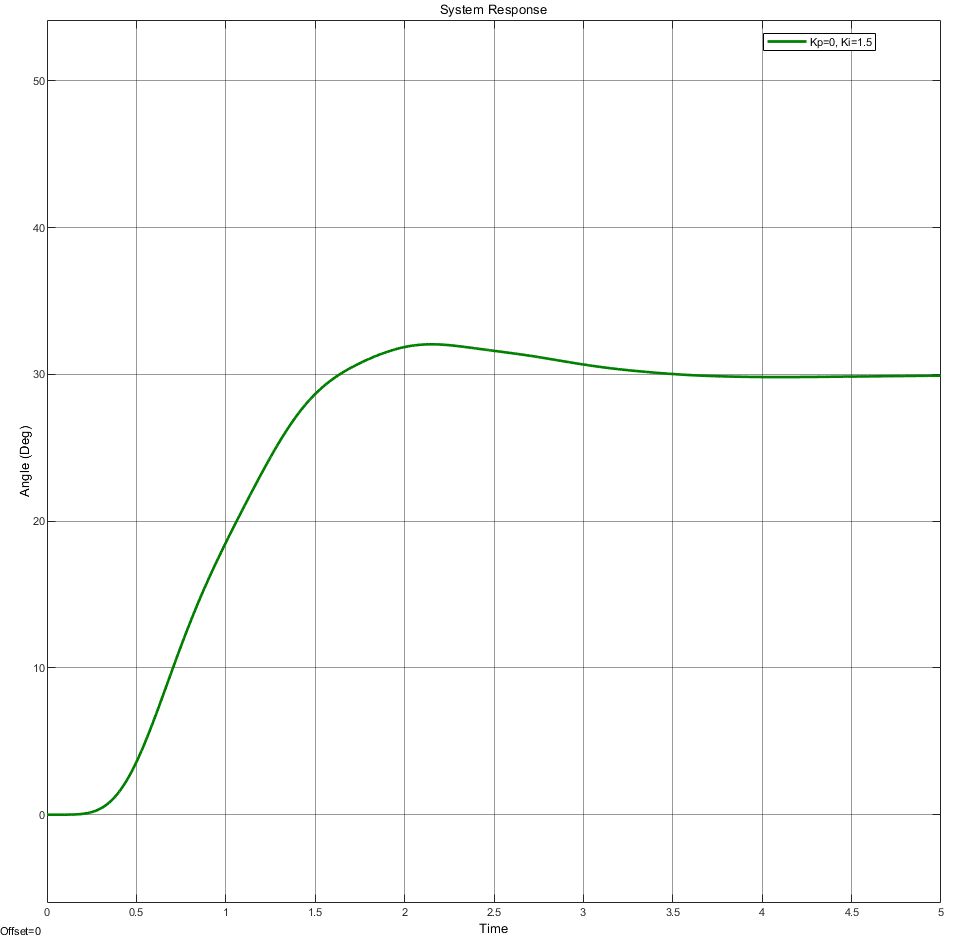
\includegraphics[width=0.3\textwidth]{inc/PI_0.png}
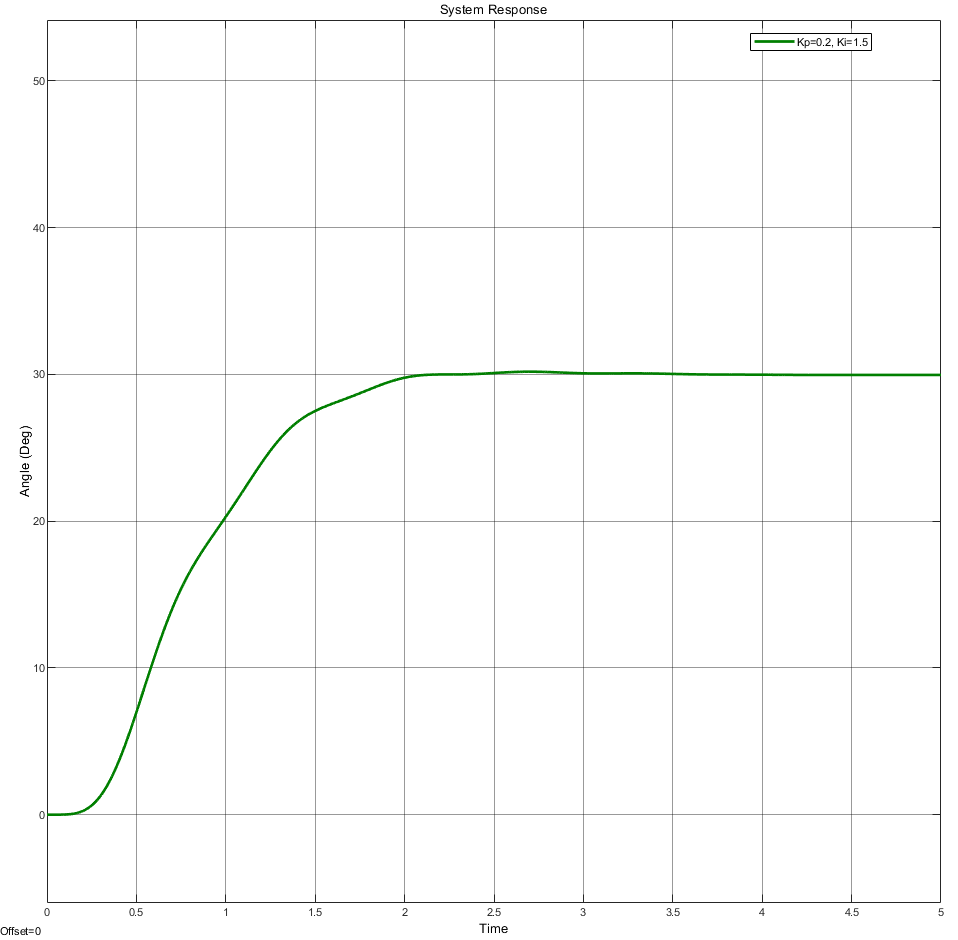
\includegraphics[width=0.3\textwidth]{inc/PI_1.png}
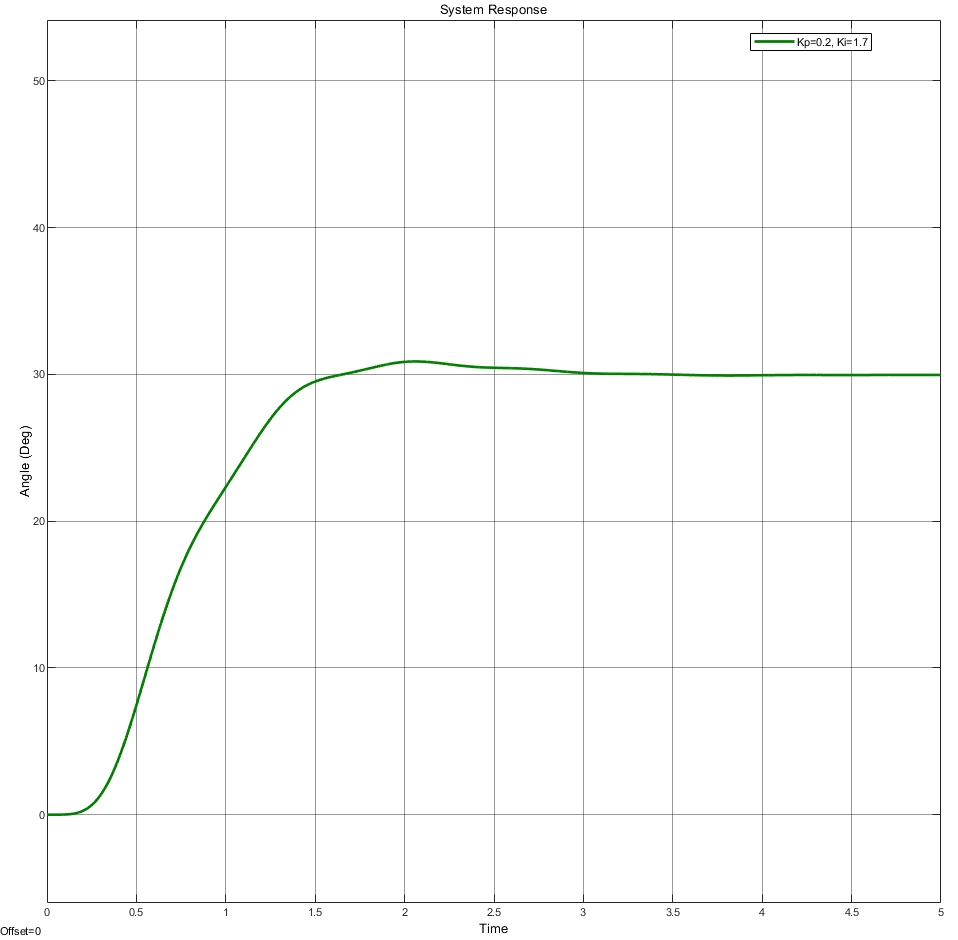
\includegraphics[width=0.3\textwidth]{inc/PI_2.png}
\begin{center}
        Figures 6,7,8 : P=[0,0.2,0.2], I=[1.5,1.5,1.7]
\end{center}

Starting with an initial P of 0 and I of 1.5 the oscillations were eliminated, and the rise speed was increased but a significant overshoot was introduced. Then slowly increasing Kp initially until overshoot was minimised but reintroduced oscillations were minor; K=0.2. Then leaving Kp and increasing Ki to speed up response, allowing for a small overshoot that the Kd can compensate for later gave a compatible range or 1.5 to 1.8. 

\newpage
\subsubsection{PD}
To tune the overshoot by responding to the rapid change and re-routing the root locus of the system toward more desired characteristics. With a negative Kd the PID compensator gain decreases when the response is changing helping to reduce oscillation by reducing the gain when the response is changing rapidly. 

{\centering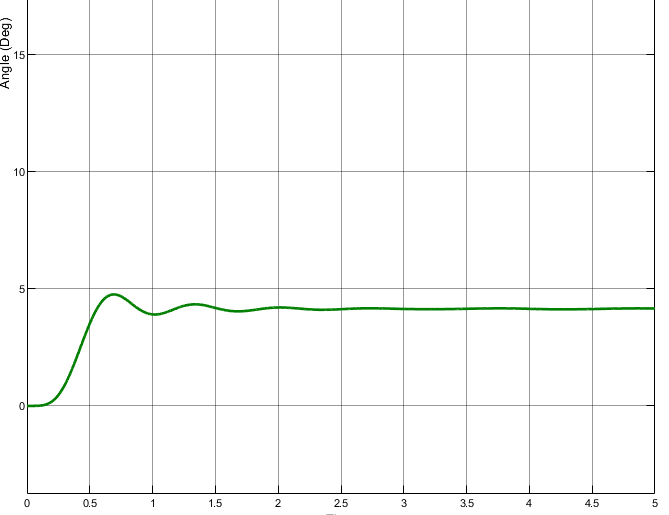
\includegraphics[width=0.33\textwidth]{inc/kd.png}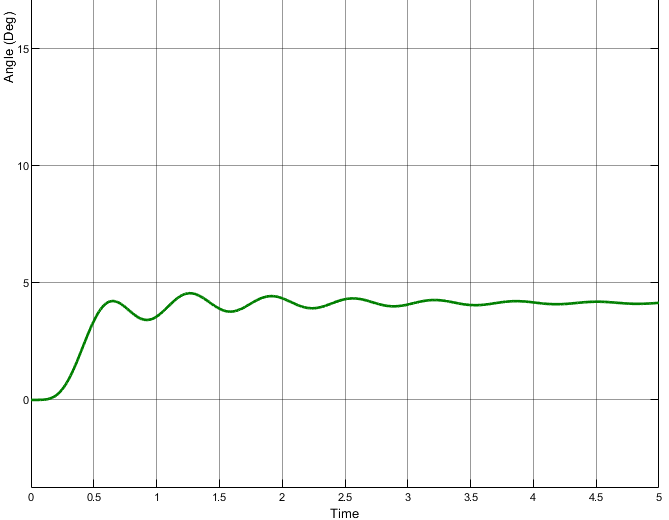
\includegraphics[width=0.33\textwidth]{inc/kd_pos.png}\\}
\begin{center}
        Figures 9. Negative Kd and Positive Kd
\end{center}

Figure 9 show both Kd compensation setting good rise characteristics but the positive exhibits greater oscillation. Both on their own have high SSE without an I term. 

\subsubsection{PID}
In combination, the three above terms are used to form the full PID block and minorly tuned exchange overshoot percentage and speed of response, by alternating I and D term values until a satisfactory characteristic response was reached. This resulted in PID of (0.2, 1.7, -0.05)

{\centering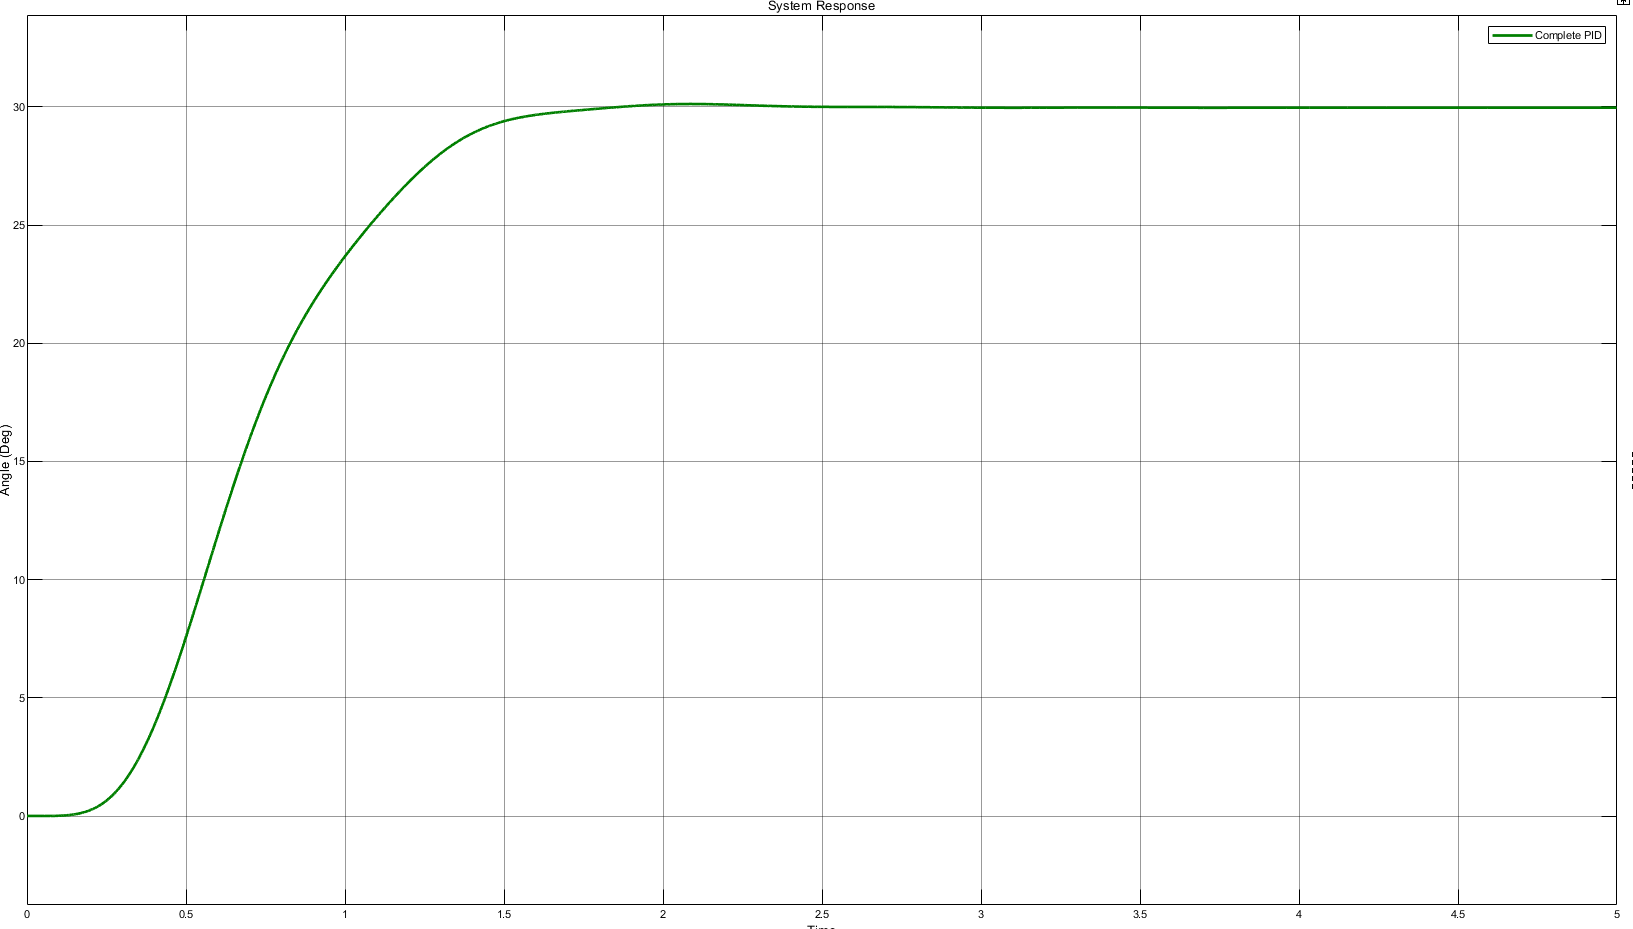
\includegraphics[width=0.5\textwidth]{inc/PID_final.png}\\}
\begin{center}
        Figure 10. Final tuned response.
\end{center}

The individualised design process before combination did most of the heavy lifting and the PID tuning was slight tuning of the values to shift response time and dampen oscillations/droop and over-undershoot. See appendix for more detailed output to tested response. Final characteristics were; approximately zero overshoot ($<0.5\%$), sub 1 second rise and settling times an heavily reduced steady state oscillation. 
 

\section{Discussion}
Throughout the calibration procedure, various linearizations were made, this introduced error and real world divergence in the model and system. The medium of simulation also has a similar effect but for what it was, it was an excellent and useful analogue.

\section{Conclusions}
In conclusions a successful PID controller was designed, tuned and implemented into the Driven Pendulum system. It had the desirable lack of overshoot, no steady state oscillations and fast response. This implementation represents a great example/learning experience for the practical application of automatized control systems and served to teach a great deal.  

\newpage
\section*{Appendices}
\subsection*{Open Loop Model}
\lstinputlisting{../lab4.m}
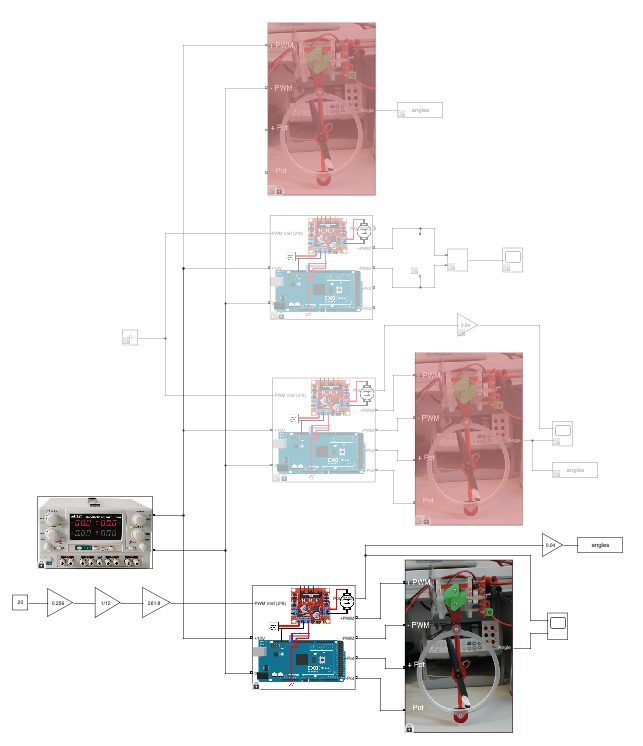
\includegraphics[width=0.9\textwidth]{inc/Lab4_sim.png}
\newpage
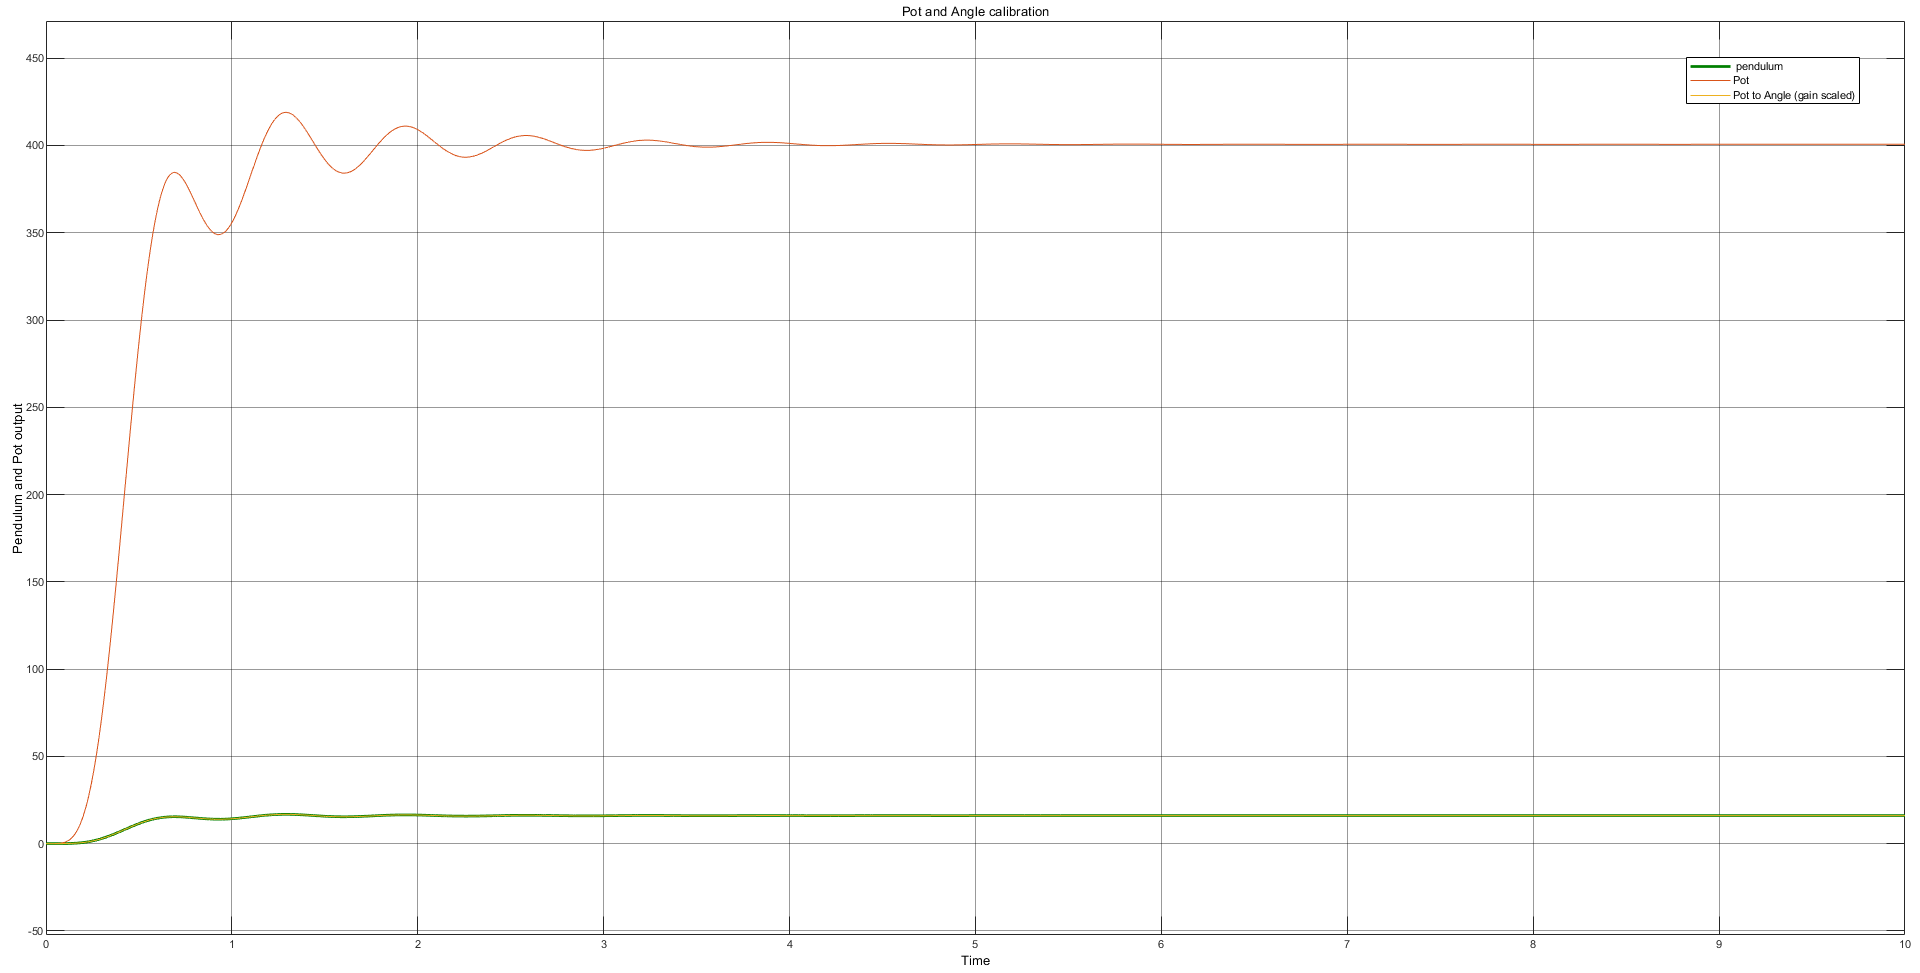
\includegraphics[width=\textwidth]{inc/pot_to_angle.png}
\begin{center}
        Pot Output vs true angle (pre gain compensator)
\end{center}
\begin{table}[h]
        \centering
        \begin{tabular}{|l|l|l|l|}
                Target & 15     & 20     & 30     \\
                SSE    & 3.0054 & 3.9729 & 6.0042
        \end{tabular}
        \caption{Target angles and resultant SSE from open loop}
\end{table}

\subsection*{P Closed Loop}

\subsection*{PID Closed Loop}
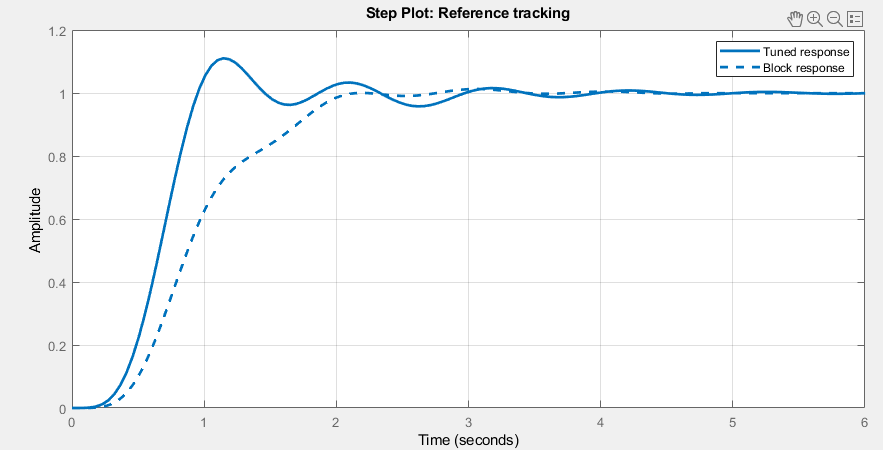
\includegraphics[width=\textwidth]{inc/lab3_reponse_PID.png}
\begin{center}
        Lab 3 TF tuning, cover range of PID values
\end{center}
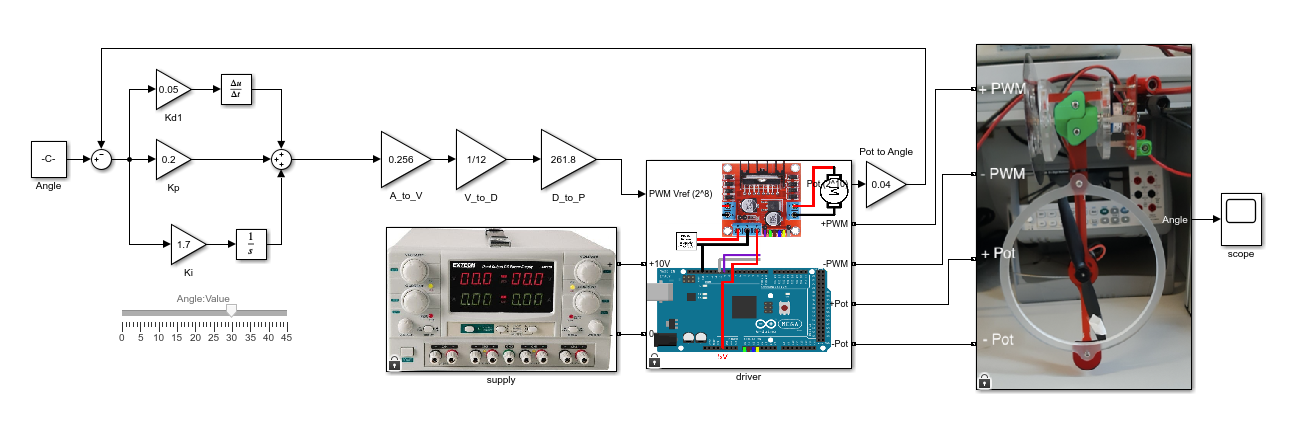
\includegraphics[width=\textwidth]{inc/PID_sim.png}
\begin{center}
        Completed Simulink PID model.
\end{center}
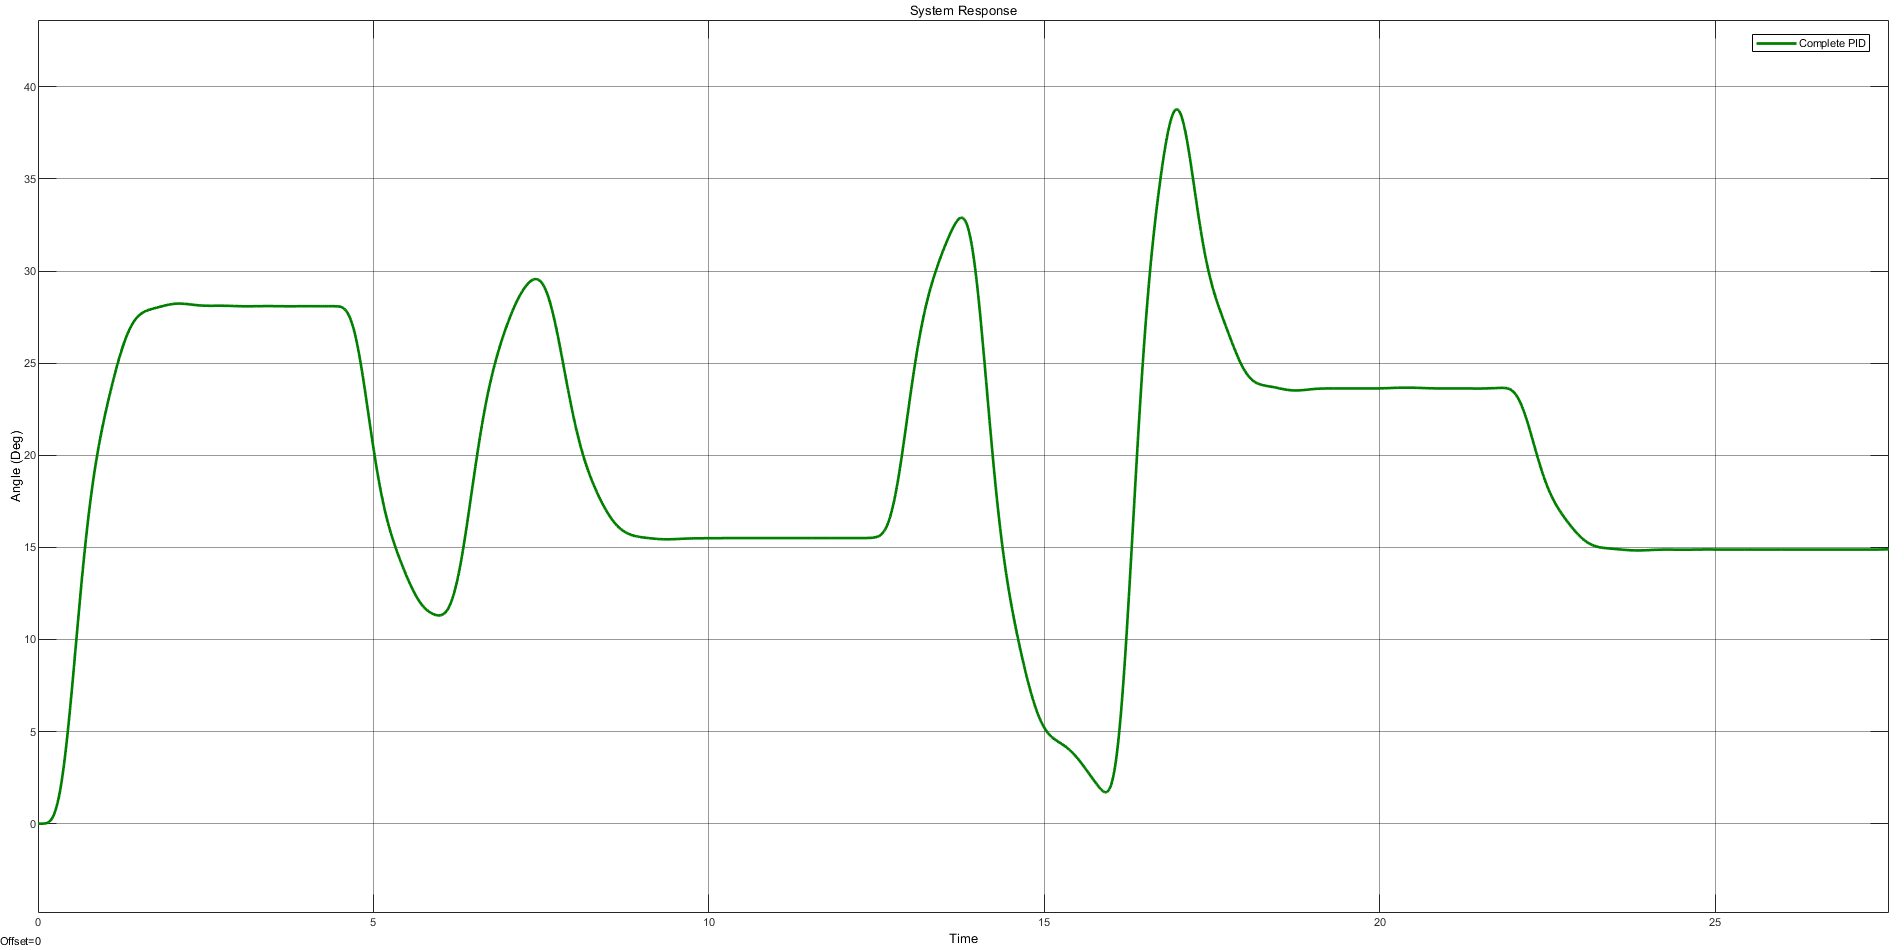
\includegraphics[width=\textwidth]{inc/pidlong.png}
    
\end{document}
